% !TEX root = ../../../I4PRJ, Grp3 - Rapport.tex
\subsection{iOS GUI}
Til iOS er der udviklet et view-lag med UIKit og C\#. Det findes i projektet Smartpool.Application.iOS.
Den visuelle implementering foretages med storyboards i Interface Builder, som er en del af Xcode-udviklingsværktøjet.

\subsubsection{Design}
I iOS applikationen designes view-klasser, der implementerer view-interfacet defineret i præsentationslaget. Brugergrænseflader på iOS platformen designes med frameworket UIKit, hvor hvert view har en tilhørende controller-klasse. Det skulle der tages højde for i designet, hvor ønsket var, at iOS designet udelukkende skulle bestå af views. Løsningen blev, at bruge UIKit controller-klasser blev brugt som broer, i mellem Smartpools præsentationslag og UIKit's view-lag. Designet er derfor lavet således, at controller-klasserne på iOS implementerer view-interfacet fra Smartpools præsentationslag.

SignUpViewBridge og StatViewBridge er de to klasser i iOS-applikationen, som implementerer hhv. ISignUpView og IStatView. Designet af de to klasser fremgår af figur~\ref{fig:ios_viewbridges}.

\begin{figure}
	\centering
	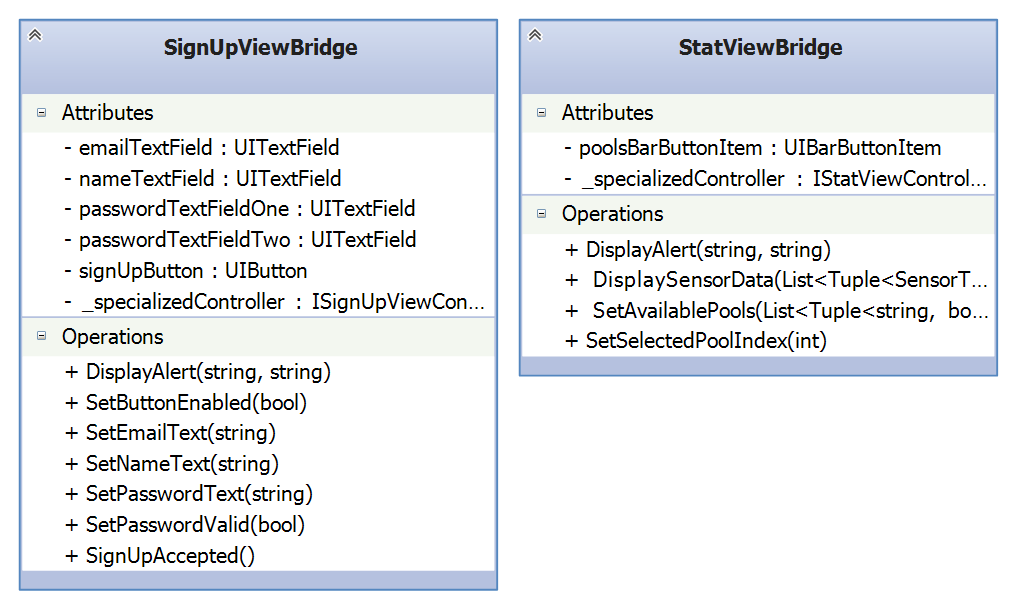
\includegraphics[width=0.7\linewidth]{figs/design/ios_viewbridges}
	\caption{SignUpViewBridge og StatViewBridge}
	\label{fig:ios_viewbridges}
\end{figure}

Udover at implementere view-interfacet, indeholder begge klasser en række UIKit elementer. Valget af user interface elementer er taget ud fra de user stories der krævede deres design.

For yderligere forklaring se dokumentation afsnit Applikationslaget under Design.